\documentclass[12pt,a4paper]{article}

% --------------------------------------------------
% Packages
% --------------------------------------------------
\usepackage[
    a4paper,
    top=25mm,
    bottom=25mm,
    left=25mm,
    right=25mm
]{geometry}

\usepackage{graphicx}
\usepackage{booktabs}
\usepackage{microtype}
\usepackage{amsmath}
\usepackage{amssymb}
\usepackage{float}
\usepackage{caption}
\usepackage{hyperref}

% --------------------------------------------------
% Hyperref Configuration
% --------------------------------------------------
\hypersetup{
    colorlinks=true,
    linkcolor=black,
    urlcolor=blue,
    pdftitle={PartnerAPI - UML Design Package},
    pdfauthor={Software Engineering Project}
}

% --------------------------------------------------
% Document Formatting
% --------------------------------------------------
\setlength{\parindent}{0pt}
\setlength{\parskip}{8pt}
\emergencystretch=3em

% --------------------------------------------------
% Title
% --------------------------------------------------
\title{
    \textbf{PartnerAPI}\\[6pt]
    \large UML Design Package
}

\author{Software Engineering Project}
\date{\today}

% --------------------------------------------------
% Document
% --------------------------------------------------
\begin{document}

\maketitle
\tableofcontents
\newpage

% ==================================================
% Architecture Overview
% ==================================================

\section{Architecture Overview}

PartnerAPI separates the public partner interface from the internal
booking platform.

The architecture follows the principle:

\begin{quote}
``Public API clients should depend on stable public contracts rather
than internal booking-system implementation details.''
\end{quote}

This separation reduces coupling between external partner
integrations and the internal booking-system implementation. It
also allows the internal booking platform to evolve without
requiring unnecessary changes to partner integrations.

% ==================================================
% Use Case Diagram
% ==================================================

\section{Use Case Diagram}

The use case model identifies the primary interactions between
partner agencies, administrators, and the PartnerAPI platform.

\begin{figure}[H]
    \centering
    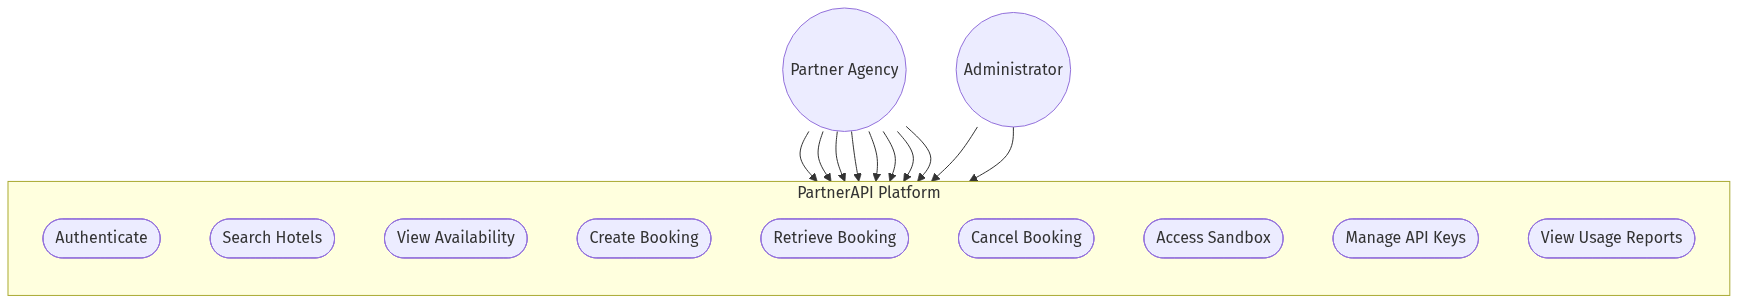
\includegraphics[
        width=\textwidth,
        height=0.65\textheight,
        keepaspectratio
    ]{../diagrams/use-case/use-case.png}
    \caption{PartnerAPI Use Case Diagram}
    \label{fig:use-case}
\end{figure}

The primary use cases represented in the system include:

\begin{itemize}
    \item Authenticate
    \item Search Hotels
    \item View Availability
    \item Create Booking
    \item Retrieve Booking
    \item Cancel Booking
    \item Access Sandbox
    \item Manage API Keys
    \item View Usage Reports
\end{itemize}

These use cases represent the principal interactions required by
external partner agencies and administrative users.

% ==================================================
% Class Diagram
% ==================================================

\section{Class Diagram}

The class diagram represents the primary domain objects and their
relationships within the PartnerAPI system.

\begin{figure}[H]
    \centering
    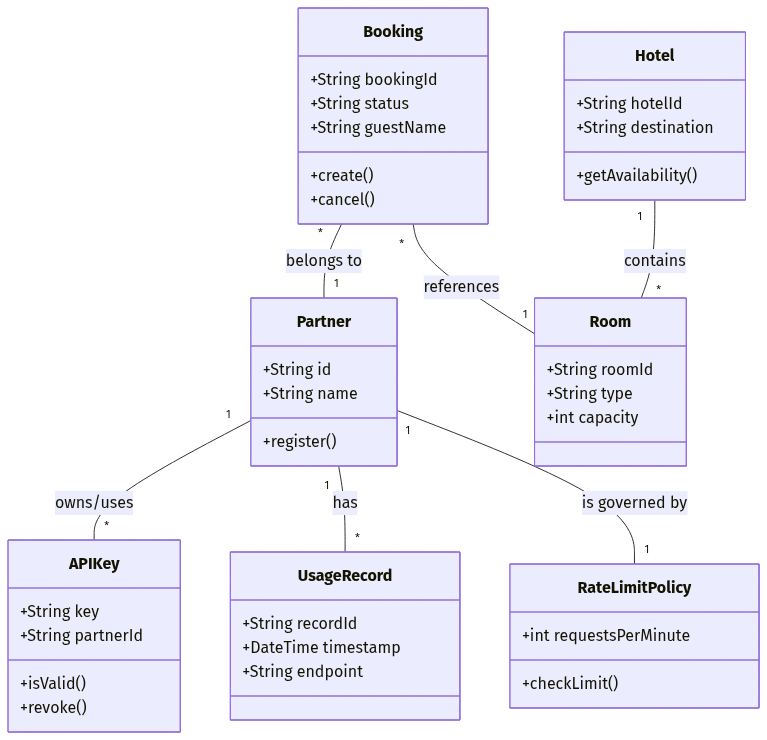
\includegraphics[
        width=\textwidth,
        height=0.65\textheight,
        keepaspectratio
    ]{../diagrams/class/class.png}
    \caption{PartnerAPI Class Diagram}
    \label{fig:class}
\end{figure}

The key domain classes include:

\begin{itemize}
    \item \textbf{Partner} -- represents a registered partner agency.
    \item \textbf{APIKey} -- represents credentials used to
    authenticate API requests.
    \item \textbf{Hotel} -- represents a hotel available through the
    booking platform.
    \item \textbf{Room} -- represents a bookable room associated with
    a hotel.
    \item \textbf{Booking} -- represents a partner-created hotel
    reservation.
    \item \textbf{RateLimitPolicy} -- defines request-rate
    restrictions for API consumers.
    \item \textbf{UsageRecord} -- records API usage for monitoring
    and reporting.
\end{itemize}

% ==================================================
% Sequence Diagram
% ==================================================

\section{Sequence Diagram}

The sequence diagram describes the ``Search and Book a Hotel Through
the API'' scenario.

The interaction begins when a partner agency submits a request to
the public API. The request is authenticated and checked against
the applicable rate-limit policy before hotel and booking services
process the request.

\begin{figure}[H]
    \centering
    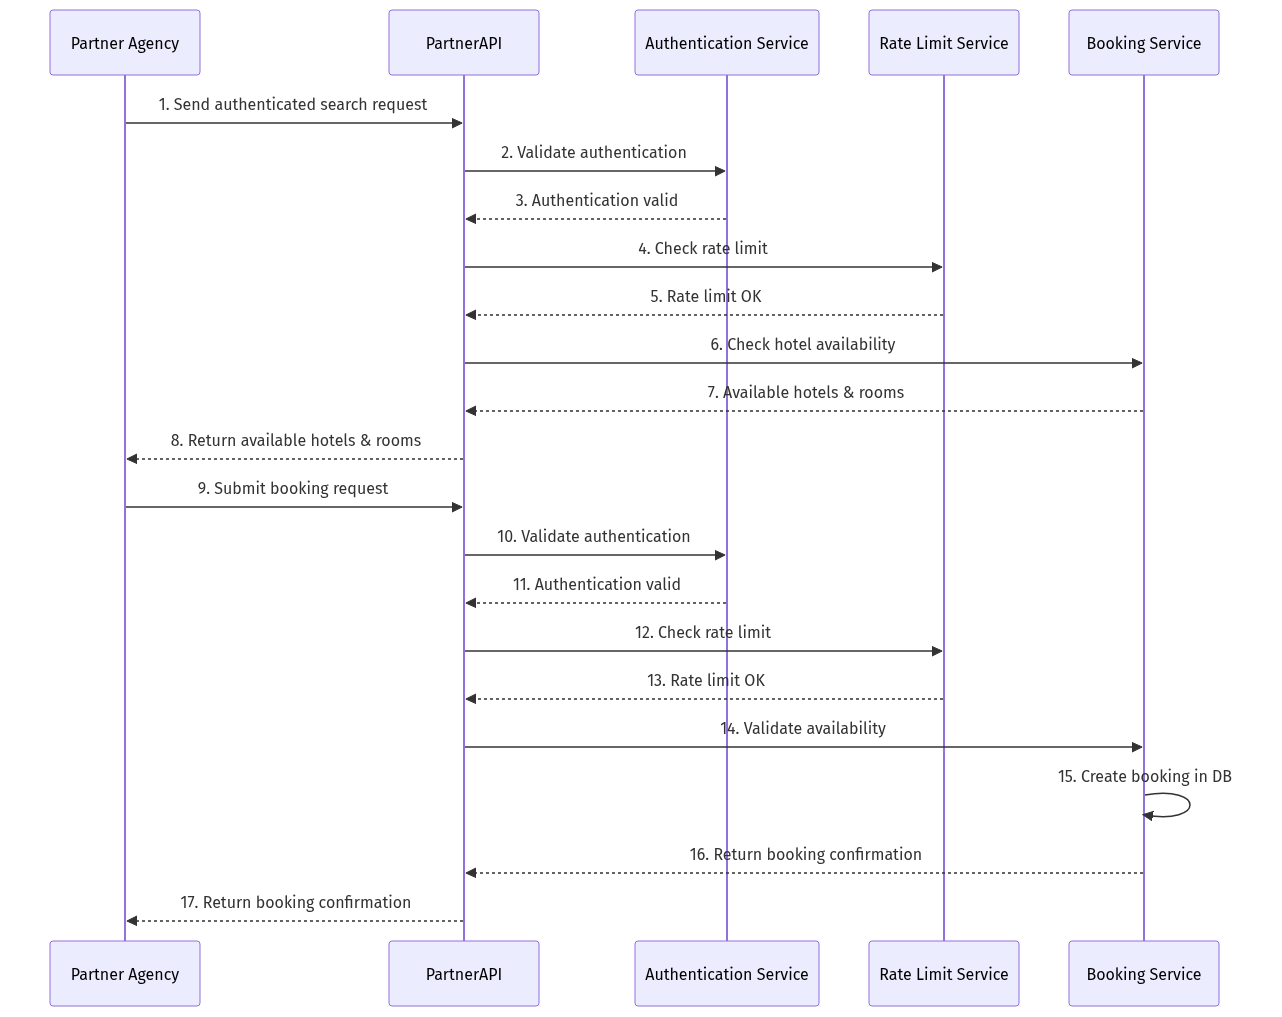
\includegraphics[
        width=\textwidth,
        height=0.65\textheight,
        keepaspectratio
    ]{../diagrams/sequence/search-book.png}
    \caption{Search and Book Hotel Sequence}
    \label{fig:sequence}
\end{figure}

The sequence illustrates the separation between the external partner
client, the public API layer, authentication and rate-limit services,
and the internal hotel and booking services.

% ==================================================
% Activity Diagram
% ==================================================

\section{Activity Diagram}

The activity diagram details the partner booking workflow from
authentication through booking confirmation.

\begin{figure}[H]
    \centering
    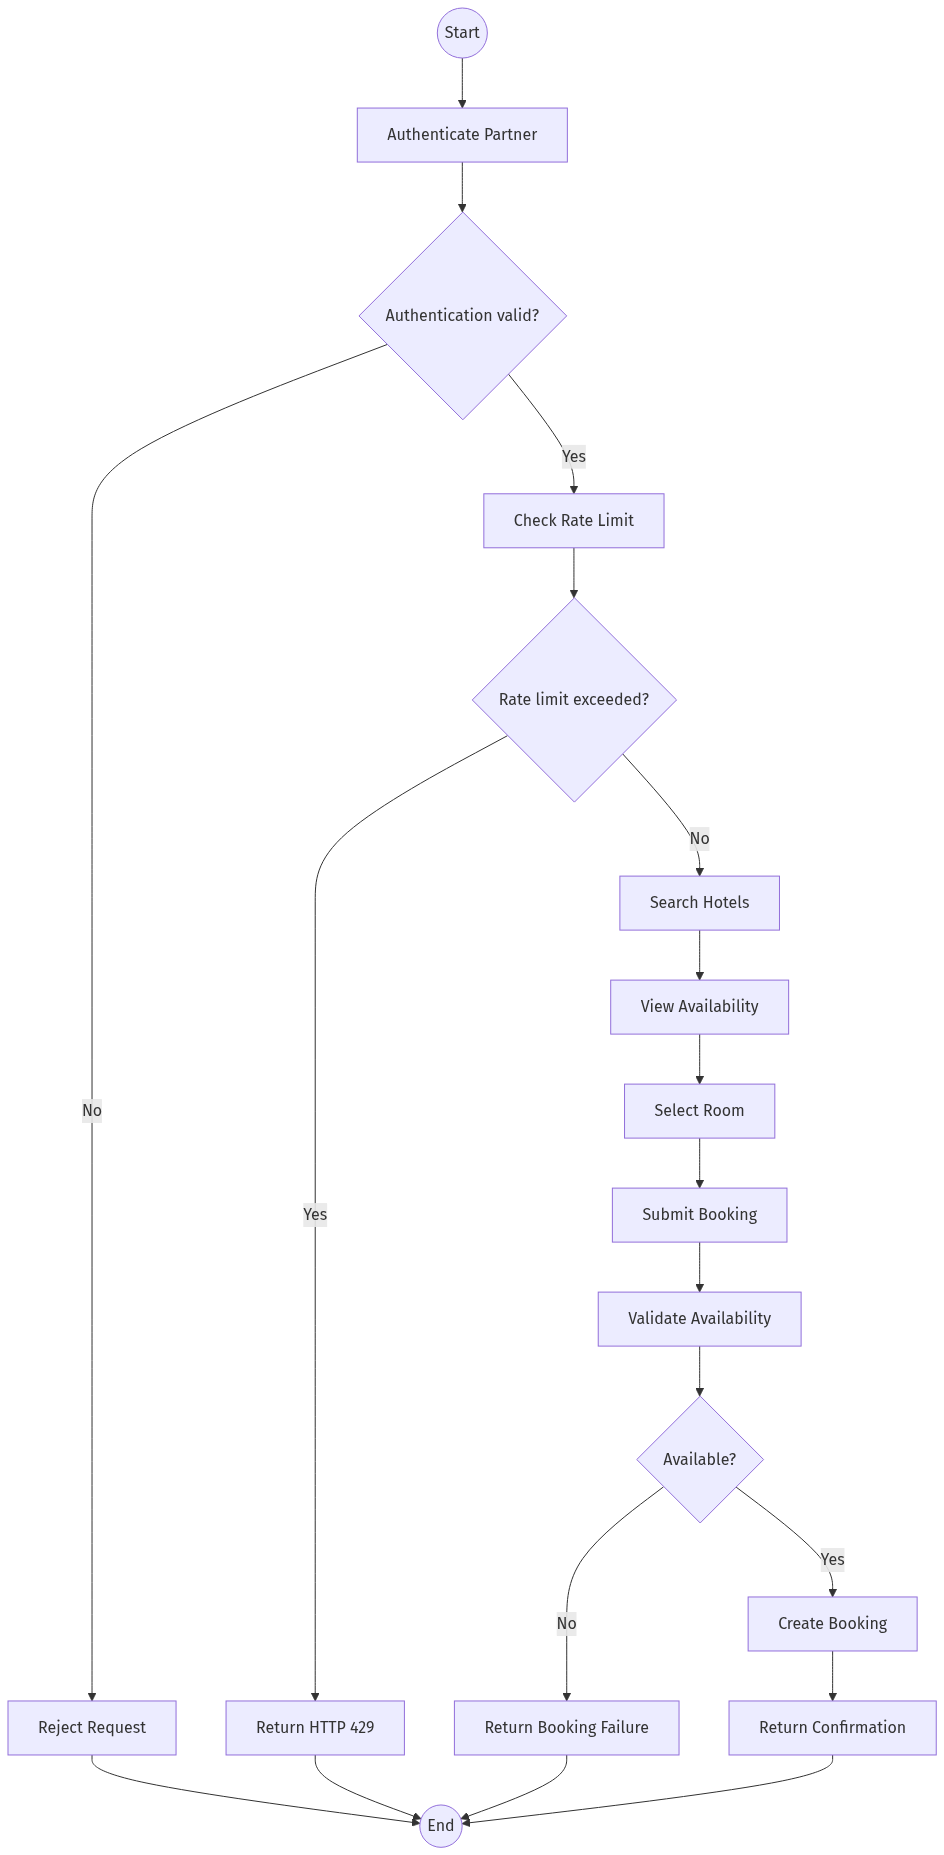
\includegraphics[
        width=\textwidth,
        height=0.75\textheight,
        keepaspectratio
    ]{../diagrams/activity/activity.png}
    \caption{Partner Booking Activity}
    \label{fig:activity}
\end{figure}

The workflow includes authentication, rate-limit validation, hotel
search, room selection, availability validation, booking creation,
and confirmation.

% ==================================================
% Booking State Diagram
% ==================================================

\section{Booking State Diagram}

A booking progresses through controlled states during its lifecycle.

\begin{figure}[H]
    \centering
    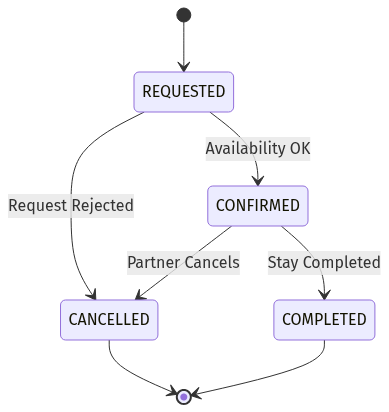
\includegraphics[
        width=0.75\textwidth,
        height=0.65\textheight,
        keepaspectratio
    ]{../diagrams/state/booking-state.png}
    \caption{PartnerAPI Booking State Diagram}
    \label{fig:booking-state}
\end{figure}

The state model provides a controlled representation of booking
lifecycle transitions. It helps ensure that booking operations are
performed only when valid state transitions are permitted.

% ==================================================
% Cohesion
% ==================================================

\section{Cohesion}

The system is organised into modules with focused responsibilities.
This promotes high cohesion because each module primarily addresses
one area of system functionality.

\begin{itemize}
    \item \textbf{Authentication module} handles authentication and
    credential validation.
    \item \textbf{Booking module} handles booking lifecycle logic.
    \item \textbf{Rate-limit module} handles API request limits.
    \item \textbf{Reporting module} handles usage and reporting data.
    \item \textbf{Partner module} handles partner configuration and
    related management operations.
\end{itemize}

Each module therefore has a focused responsibility, reducing
unnecessary dependencies between unrelated areas of the system.

% ==================================================
% Coupling
% ==================================================

\section{Coupling}

The public API is separated from the internal booking
implementation.

The API communicates through stable service interfaces rather than
directly depending on internal database structures. This reduces
coupling between the external partner integrations and the internal
booking platform.

As a result, the internal booking platform can evolve without
forcing partners to modify their integrations unnecessarily,
provided that the public API contracts remain stable.

% ==================================================
% Design Rationale
% ==================================================

\section{Design Rationale}

The UML design follows several software engineering principles:

\begin{itemize}
    \item \textbf{High cohesion} -- each module has a focused
    responsibility.
    \item \textbf{Low coupling} -- external partners depend on stable
    API contracts rather than internal implementation details.
    \item \textbf{Stable API contracts} -- public interfaces are
    separated from internal booking implementation.
    \item \textbf{Clear responsibility boundaries} -- authentication,
    booking, rate limiting, partner management, and reporting have
    distinct responsibilities.
    \item \textbf{Independent testing} -- separated components can be
    tested with focused test cases.
    \item \textbf{Controlled change} -- changes to internal
    implementation can be made with reduced impact on external
    partner integrations.
\end{itemize}

% ==================================================
% Conclusion
% ==================================================

\section{Conclusion}

The UML design package defines the architecture and behavioural
structure of PartnerAPI through use case, class, sequence, activity,
and state diagrams.

The design separates the public API from the internal booking
platform while maintaining clear responsibility boundaries. High
cohesion within modules and low coupling between external partners
and internal implementation support maintainability, independent
testing, and controlled system evolution.

Overall, the UML models provide a consistent structural and
behavioural representation of the PartnerAPI system and support the
project's objective of enabling partner agencies to integrate with
the hotel booking platform through a stable public API.

\end{document}